
\centering

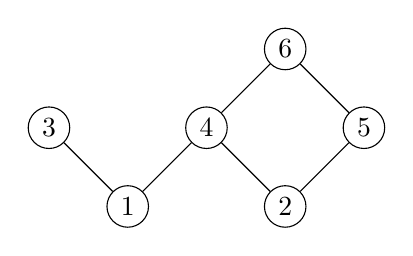
\begin{tikzpicture}
  [scale=1.0,auto=left,every node/.style={circle, draw, color=black!100, inner sep=0pt, minimum width=15pt}]

 \node (n1) at (1,0) {$1$};
 \node (n2) at (3,0) {$2$};
 \node (n3) at (0,1) {$3$};
 \node (n4) at (2,1) {$4$};
 \node (n5) at (4,1) {$5$};
 \node (n6) at (3,2) {$6$};

 \foreach \from/\to in {n1/n3, n1/n4, n2/n4, n2/n5, n4/n6, n5/n6}
   \draw (\from) -- (\to);

\end{tikzpicture}
\caption{The Hasse diagram of a poset.}